% Section 5 -- drafted by Claude (2026-10-21), revised after review. Numbers from scripts/report_results.py.
\section{Results}\label{sec:results}

\paragraph{Offline.}
Table~\ref{tab:offline} follows the versions through the three settings of Section~\ref{sec:data}. In the default setting V1 scored about the same as the baseline ($-0.0003$, SE 0.0011), and setting $\lambda$ to 0 for V3 cost $+0.00300$ (SE 0.00047). In the hidden-sized setting, pooling difficulties from one partner pair helped a little on each of the four benchmarks with partner pairs ($-0.00116$, SE 0.00015), assuming, as my harness does, that each pair's items are split independently; with one split shared by every subject on a benchmark the gain was $-0.00007$ (SE 0.00005). The large offline gains came from the two LLM inputs, testable only in the rated setting. The difficulty ratings gave $-0.0144$ (SE 0.0011), $-0.0144$ (SE 0.0009) and $-0.0141$ (SE 0.0008) with one and two partner pairs, and $-0.0140$ (SE 0.0010) and $-0.0097$ (SE 0.0007) with only 90\% or 70\% of items rated. The guesses gave another $-0.0135$ (SE 0.0013), $-0.0132$ (SE 0.0012) with one or two partner pairs, and beat V4 on each held-out benchmark ($-0.0077$ on MathArena, $-0.0217$ on Multi-SWE-bench, $-0.0101$ on REAL and $-0.0109$ on ResearchCodeBench). The submission folders gave a similar gain in-sample (Appendix~\ref{app:engineering}).

\begin{table}[t]
  \caption{Offline Brier ALC (lower is better) in three settings, pooled over seeds 0--2. $\Delta$ is a row's score minus the score of the row above it on the same pair results (negative favors the row); the SE treats each subject--benchmark pair as a cluster. Blocks use different pairs, so their scores and differences cannot be added. V3 is worse than V1 and V2 offline in every block where they meet; I adopted it because of formative feedback (Appendix~\ref{app:rules}).}
  \label{tab:offline}
  \centering
  \small
  \begin{tabular}{lrrr}
\toprule
Predictor & Pair results & Brier ALC & $\Delta$ to row above (SE) \\
\midrule
\multicolumn{4}{l}{\emph{Default setting, $K = 0$}} \\
\quad Baseline & 576 & 0.2161 & -- \\
\quad V1 ($\lambda = 0.5$) & 576 & 0.2158 & $-0.0003$ (0.0011) \\
\quad V3 ($\lambda = 0$) & 576 & 0.2188 & $+0.00300$ (0.00047) \\
\addlinespace
\multicolumn{4}{l}{\emph{Hidden-sized setting, $K = 1$}} \\
\quad V1 ($\lambda = 0.5$) & 471 & 0.1959 & -- \\
\quad V2 ($\lambda = 0.5$, pooling) & 471 & 0.1948 & $-0.00116$ (0.00015) \\
\quad V3 ($\lambda = 0$, pooling) & 471 & 0.1993 & $+0.00459$ (0.00055) \\
\addlinespace
\multicolumn{4}{l}{\emph{Rated setting, $K = 0$}} \\
\quad V3 & 594 & 0.2074 & -- \\
\quad V4 (ratings, $t = 0.5$, gate) & 594 & 0.1930 & $-0.0144$ (0.0011) \\
\quad V5 (V4 + subject guesses, $t_g = 0.75$) & 594 & 0.1795 & $-0.0135$ (0.0013) \\
\bottomrule
\end{tabular}

\end{table}

Most of V5's gain comes at the first budgets (Figure~\ref{fig:budgets}). At budget 0 V4 predicts 0.5 everywhere and scores 0.2500, against V5's 0.2037. Weighted as in Eq.~\eqref{eq:alc}, budgets 0 and 1 give 74\% of V5's gain over V4 and budget 3 another 17\%, and by budget 31 the two curves meet.

\begin{figure}[t]
  \centering
  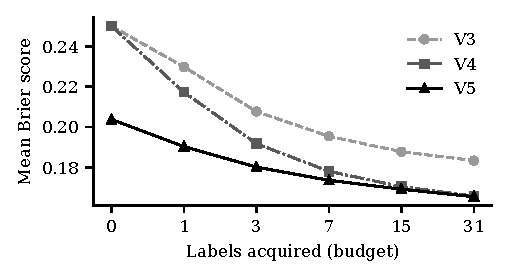
\includegraphics[width=0.56\linewidth]{figures/budgets}
  \caption{Mean Brier score at each budget in the rated setting with no partner pairs (594 pair results; budgets on a $\log_2(1 + b)$ axis). V4's ratings act from budget 1 on and grow with the labels; V5's guesses act from budget 0 and matter most before the first few labels.}
  \label{fig:budgets}
\end{figure}

I chose both trust levels to limit the damage if the LLM inputs do not transfer. At trust levels 0, 0.25, 0.5, 0.75 and 1, the worst-case regret was 0.0188, 0.0096, 0.0065, 0.0142 and 0.0236 for the rating trust $t$ and 0.0148, 0.0094, 0.0049, 0.0013 and 0.0108 for the guess trust $t_g$. At $t_g = 0.75$, V5 still beat V4 when the held-out benchmark's guesses were shuffled among its subjects ($-0.0024$, SE 0.0020), raised by one logit ($-0.0045$, SE 0.0013) or lowered by one ($-0.0126$, SE 0.0019). These scenarios are milder than what happened to the metadata priors on Codabench. Shuffling keeps the benchmark's average level: Multi-SWE-bench, which gives 57\% of V5's gain, still gained 0.0107 with shuffled guesses, while MathArena lost 0.0081. No scenario in the rule combined a shuffle with a shift or reversed the guesses; computed afterwards, either case makes V5's budget-0 Brier worse than 0.25, by 0.006 for shuffled guesses moved up one logit and by 0.021 for reversed ones.
\paragraph{Formative feedback.}
Table~\ref{tab:formative} lists the upload of each version; the probes of Appendix~\ref{app:engineering} are left out. Each row comes from its own draw (Section~\ref{sec:data}), so differences between rows mix version and draw, and I use two quantities that depend less on the draw. A version that predicts one value $p$ for every item of a pair at budget 0 has Brier score $(p - \bar y)^2 + \bar y(1 - \bar y)$ and calibration error $|p - \bar y|$, where $\bar y$ is the pair's success rate; the Brier score minus the squared calibration error recovers the floor $\bar y(1-\bar y)$, which I subtract from the score to discount easy draws. And since V3 and V4 predict exactly 0.5 at budget 0, their budget-0 Brier is 0.25 on any draw, a fixed reference for later versions.

\begin{table}[t]
  \caption{Formative Codabench results, each a single draw (UTC+8 dates). Score: mean Brier ALC over the draw's pairs. Floor: the draw's mean $\bar y(1-\bar y)$ recovered from the budget-0 rows, so score $-$ floor discounts easy draws (SE over pairs; approximate for V5, whose first budget-0 predictions may have come before the guess arrived). The first row is a constant 0.5.}
  \label{tab:formative}
  \centering
  \small
  \setlength{\tabcolsep}{4pt}
  \begin{tabular}{llcrrrr}
\toprule
Codabench & Date & Version & Pairs & Score & Budget-0 Brier & Score $-$ floor (SE) \\
\midrule
951242 & 2026-09-29 & constant 0.5 & 8 & 0.2500 & 0.250 & 0.078 (0.022) \\
954621 & 2026-10-01 & Baseline & 9 & 0.2322 & 0.298 & 0.048 (0.013) \\
958131 & 2026-10-03 & V1 & 9 & 0.2025 & 0.283 & 0.036 (0.011) \\
963204 & 2026-10-06 & V2 & 8 & 0.1877 & 0.303 & 0.045 (0.011) \\
963789 & 2026-10-06 & V3 & 9 & 0.1559 & 0.250 & 0.034 (0.008) \\
968769 & 2026-10-08 & V4 & 8 & 0.1704 & 0.250 & 0.031 (0.011) \\
1005477 & 2026-10-20 & V5 & 8 & 0.1408 & 0.180 & 0.009 (0.007) \\
\bottomrule
\end{tabular}

\end{table}

The baseline, V1 and V2 all scored worse than 0.25 at budget 0 (0.298, 0.283 and 0.303), although offline they had been below it (0.244 and 0.238 for the baseline and V1 in the default setting, 0.232 for V2 in the hidden-sized one). On the hidden benchmarks their metadata priors put budget-0 predictions further from the pairs' success rates than 0.5 was, so I switched to V3. V5's budget-0 Brier was 0.180 on 8 pairs, below 0.25 on 6 of them. By the rule I committed before uploading it (Appendix~\ref{app:rules}), V5 replaced V4 as the final entry. Its score net of the floor, 0.009 (SE 0.007), is the lowest of all uploads; V4's was 0.031 (SE 0.011). With one draw per version and standard errors this wide, I read the formative results as consistent with the offline ones, not as a separate measure.
